\chapter{Empirical Analysis}
\label{chap:empirical_analysis}

\section{The Geography of Intermediaries}
\label{sec:geographical_specialisation}

This section delves into the geographical patterns exhibited by intermediaries, focusing on the locations of the entities they service and the jurisdictions they select to incorporate in. First, an overview of the location of entities, officers and intermediaries is provided. Then, examining specialization at the country level, analyzing how intermediaries based in specific nations in the aggregate, are concentrated in different and distinct countries. Lastly, we shift to the individual intermediary level to investigate the concentration of their client networks and jurisdictional preferences.

\subsubsection{Concentration of Entities, Intermediaries, and Officers}

\label{subsubsec:concentration_elements}

\begin{figure}[htbp]
    \centering
    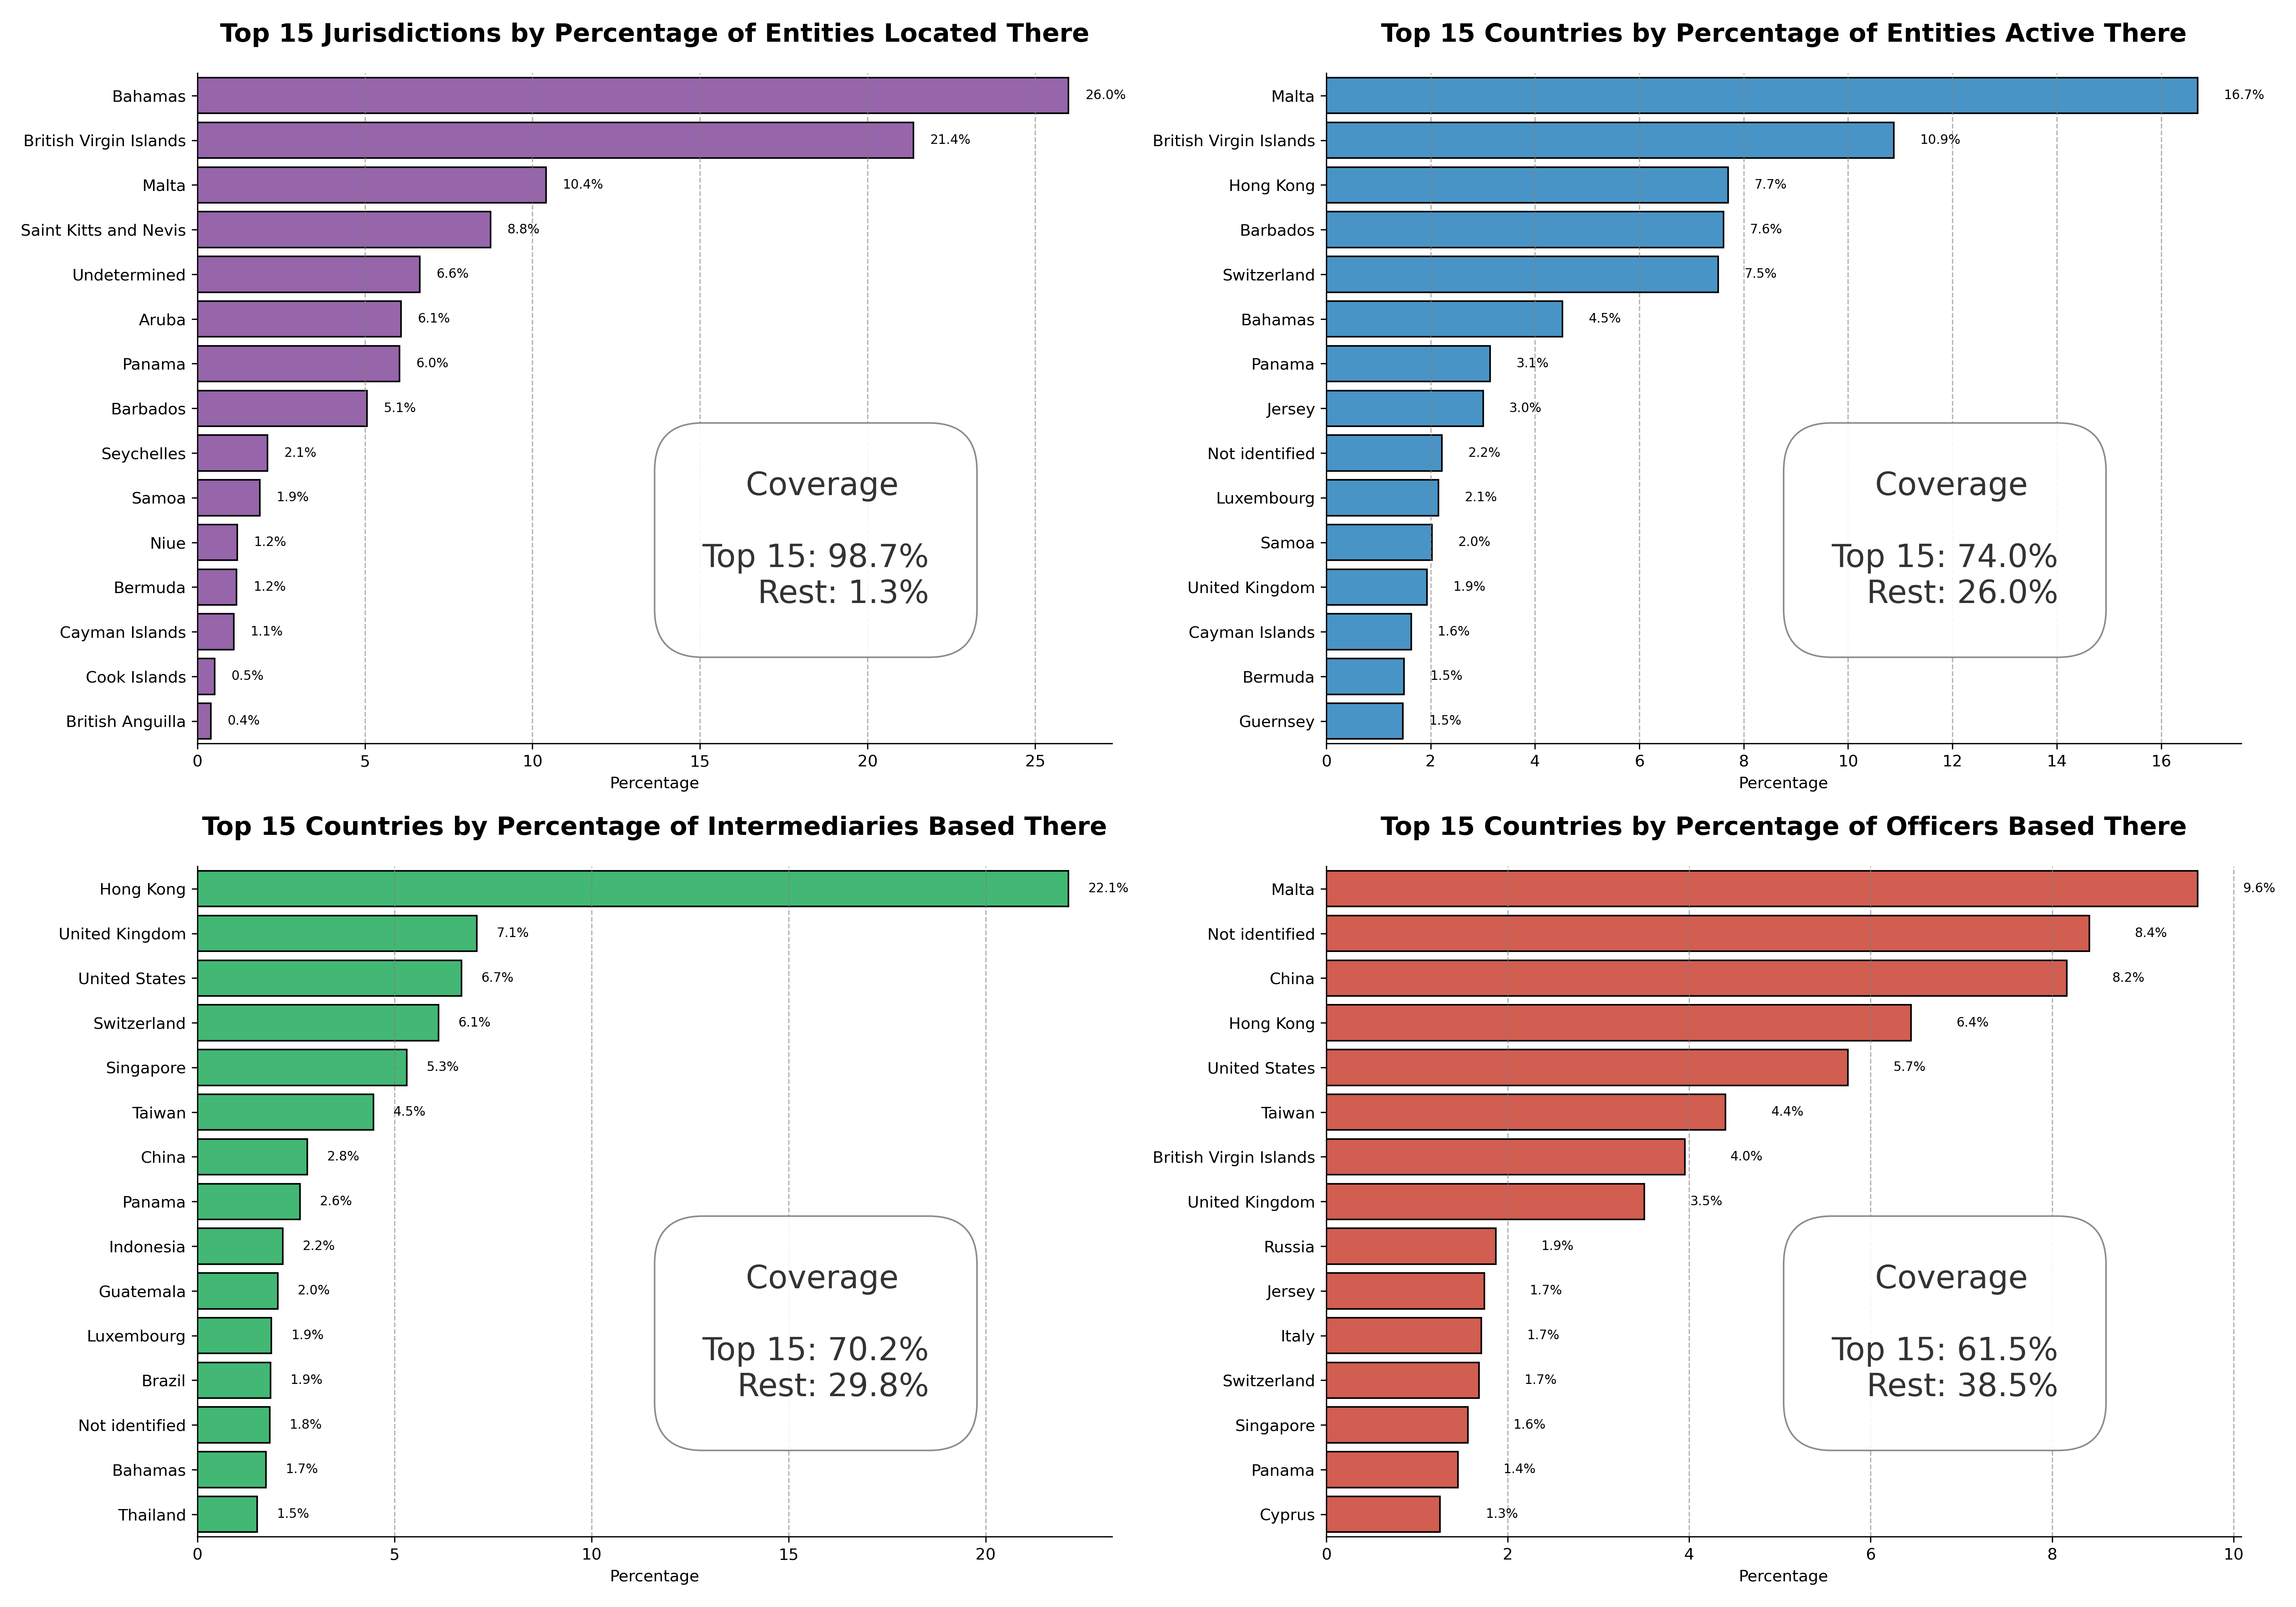
\includegraphics[width=0.9\textwidth]{images/Preliminary_Geography_Overview.png} 
    \caption{Geographical Concentration of Entities, Intermediaries, and Officers}
    \label{fig:preliminary_geography_overview}
\end{figure}

A striking initial observation is the pronounced geographical concentration inherent in offshore financial activities, a characteristic that permeates all primary node types: entities, intermediaries, and officers.

While the dataset encompasses a vast network spanning over 200 countries and territories, these structures appear to be disproportionately concentrated within a relatively small cohort of key and recurring locations. Approximately 98.7\% of all entities within the dataset are registered in just 15 jurisdictions (see Figure \ref{fig:preliminary_geography_overview}, top-left panel). This aligns with the literature, such as Laffitte (2024), which suggests that Offshore Financial Centers (OFCs) often develop specialized expertise in particular 'legal technologies'-be it specific corporate vehicles like International Business Companies (IBCs), banking secrecy laws, or tax-exempt trusts. The British Virgin Islands, Panama, and the Bahamas, for instance, emerge as clear leaders in this regard, collectively accounting for a substantial majority of entity incorporations in the dataset.

This pattern of concentration, however, is not confined to the legal domiciliation of entities; it extends to the operational footprint of these entities and the intermediaries. As seen in the top-right panel, approximately 74\% of entities have their operational activities linked to the top 15 countries. These countries differ drastically, though, from the primary incorporation jurisdictions, featuring primarily the major financial centers such as Malta, Hong Kong, the United Kingdom, Switzerland, and Cyprus. This is to be expected as these same countries are highly linked to multinationals' tax avoidance. Malta and Hong Kong, for example, which rank first and second respectively for entity activity, also have exceptionally high ratios of corporate income tax revenues to national income, Malta being the highest, Hong Kong third (Saez and Zucman, 2019). 

The concentration extends to the intermediaries. The bottom-left panel of Figure \ref{fig:preliminary_geography_overview} shows that approximately 70.2\% of intermediaries are based in the top 15 countries. These include prominent financial centers like Hong Kong, the United Kingdom, Switzerland, the United States, and China. This resonates with the previously cited findings of Stausholm and Garcia-Bernardo (2024), who argue that the professional services underpinning the offshore world, tend to cluster in major global financial centers rather than exclusively in traditional tax havens. These hubs provide the necessary infrastructure, talent pool, and network access for intermediaries to orchestrate these structures.

Finally, the bottom-right panel indicates that around 61.5\% of officers are associated with the top 15 countries, with Hong Kong, China (excluding Hong Kong), the United Kingdom, Taiwan, and the United States being particularly prominent. As with intermediaries, this suggests that the individuals who hold positions of control or influence within these offshore entities are often based in the same major financial centers.

The varying degrees of concentration across these node types are also worth pointing out. The near-total concentration of entity incorporations (98.7\% in the top 15) contrasts with the more diffuse, yet still significant, concentration for active entities (74.0\%), intermediaries (70.2\%), and officers (61.5\%). This suggests that while the legal creation of offshore entities is highly centralized in a few specialized jurisdictions, the operational management, facilitation, and beneficial control of these entities are spread across a wider, though still limited, range of influential countries. This has both implications for what \textit{type} of chokepoints exist as well as to which \textit{extent}.


\subsubsection{Intermediary Specialisation at the Country Level}
\label{subsubsec:intermediary_specialisation_country}

To understand how intermediaries based in specific countries orient their services, we examine two key dimensions: the geographical distribution of countries where the entities are primarily active, and the jurisdictions they predominantly use for incorporating these entities. Heatmaps are used to visually represent these patterns for intermediaries headquartered in the top 5 countries by intermediary count within the dataset: Hong Kong (HKG), Great Britain (GBR), the United States (USA), Switzerland (CHE) and Singapore (SGP). The rest of the top 15 (thus accounting for 70.2\% of all intermediaries as aforementioned) are left in the appendix, as well as Cyprus to illustrate the well-known Russia-Cyprus corridor, and how they manifest themselves in figures like these (e.g. ICIJ, n.d.; Garcia-Bernado et al., 2017) 

Figures \ref{fig:geography_country_heatmaps_top5} display these heatmaps. Each panel within these figures corresponds to one of the top 5 intermediary home countries. The top bar in each panel illustrates the percentage distribution of client entities' countries of activity, while the bottom bar shows the percentage distribution of jurisdictions used for entity incorporation by intermediaries based in that home country. Darker shades indicate higher concentrations. Alongside each panel, normalized Shannon entropy values are provided for client country concentration ($H_c$) and incorporation jurisdiction concentration ($H_j$), where a value closer to 0 indicates higher concentration (less diversity) and a value closer to 1 indicates greater diversity. Common across all of them in this figure is being major global and regional financial centres.

\begin{itemize}
    \item \textbf{Hong Kong (HKG):} Intermediaries in Hong Kong predominantly serve entities active within Hong Kong itself (63\%), with a significant portion also linked to China (35\%). This strong domestic and near-regional focus ($H_c=0.23$) contrasts with their incorporations. For incorporations, the British Virgin Islands (VGB) is overwhelmingly favored (78\%), followed by Samoa (WSM, 7\%) and the Cayman Islands (CYM, 6\%), resulting in a jurisdiction entropy ($H_j=0.33$) that, while still concentrated, indicates slightly more diversity than their client base. This pattern suggests HKG intermediaries leverage specific offshore jurisdictions like VGB for their largely local and Chinese clientele. In other words, a corroboration that Hong Kong intermediaries act as a gateway for Chinese to access offshore structuring (see, for example, Wei, 2024).

    \item \textbf{Great Britain (GBR):} UK-based intermediaries also show a strong domestic client focus (GBR, 73\%), with smaller but notable client links to Crown Dependencies like Jersey (JEY, 6\%). Their client country entropy ($H_c=0.37$) is relatively low. For incorporations, they too heavily rely on VGB (66\%), followed by Panama (PAN, 15\%) and the Bahamas (BHS, 13\%), yielding a jurisdiction entropy ($H_j=0.35$) similar to their client concentration. This suggests a model of serving primarily UK-based clients using a select few popular offshore jurisdictions.

    \item \textbf{United States (USA):} US-based intermediaries exhibit a very strong domestic client focus (USA, 71\%), with a low client country entropy ($H_c=0.24$). Their preferred incorporation jurisdictions are VGB (43\%), Panama (PAN, 19\%), and the Cook Islands (COK, 18\%), showing more jurisdictional diversity ($H_j=0.50$) than their client base. 

    \item \textbf{Switzerland (CHE):} Swiss intermediaries show an exceptionally high concentration of domestic clients (CHE, 94\%), reflected in a very low $H_c=0.11$. This aligns with Switzerland's role as a wealth management hub primarily serving its own residents or those with assets managed through Swiss institutions. For incorporations, Panama (PAN, 50\%) and VGB (32\%) are dominant, leading to a moderate jurisdiction entropy ($H_j=0.45$).

    \item \textbf{Singapore (SGP):} Intermediaries in Singapore serve a mix of domestic (SGP, 47\%) and regional clients, particularly from Indonesia (IDN, not in top 5 shown but a known link). Their client country entropy ($H_c=0.32$) is moderate. Like Hong Kong, they overwhelmingly prefer VGB (84\%) for incorporations, resulting in a low jurisdiction entropy ($H_j=0.26$).
\end{itemize}

\begin{figure}[htbp]
    \centering
    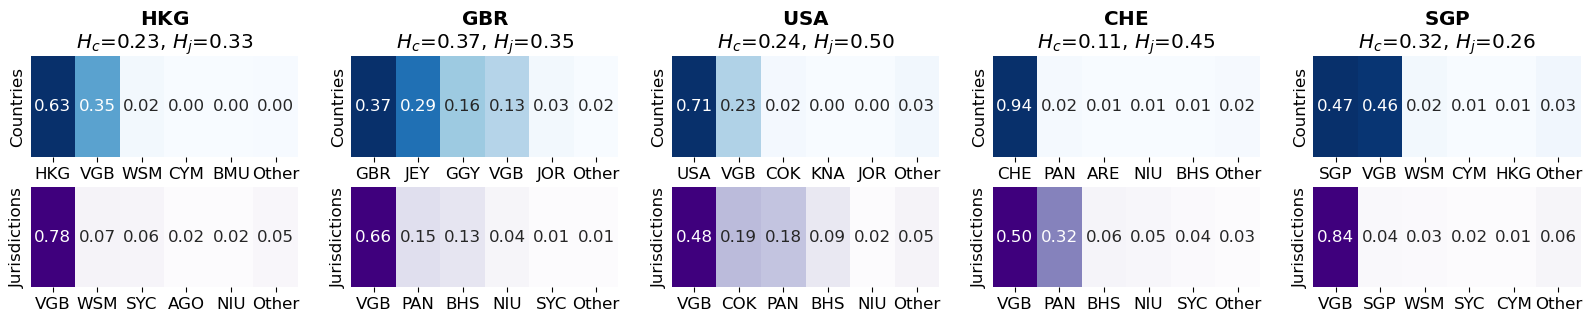
\includegraphics[width=0.9\textwidth]{images/Geography_Country_Heatmaps_Top5.png}
    \caption{Client and Incorporation Jurisdiction Heatmap for Intermediaries in Top 5 Countries (HKG, GBR, USA, CHE, SGP)}
    \label{fig:geography_country_heatmaps_top5}
\end{figure}

Across these five countries, a general trend emerges: intermediaries often have a geographically concentrated client base, frequently dominated by entities active in their own country of operation or in close regional proximity. However, their choice of incorporation jurisdictions tends to be more outwardly focused, though often dominated by a few key OFCs like the British Virgin Islands, Panama, and Seychelles. This suggests that while client acquisition may be localized or regionally focused, intermediaries draw from a global "market for tax havens" to select specific "legal technologies" offered by these jurisdictions to meet diverse client structuring needs (Laffitte, 2024). 

This observed difference in diversification is quantified by comparing the normalized entropy of jurisdictions used for incorporation ($H_j$) with the normalized entropy of client entity countries ($H_c$) at the aggregate level for intermediaries in all countries. Figure \ref{fig:geography_country_level_entropy_distribution} displays the distributions of these two entropy measures. The distribution of jurisdiction entropy (purple curve) is visibly to the right compared to the distribution of client country entropy (blue curve). A higher entropy value indicates greater diversification. Given we are comparing two distributions, a two-sample Kolmogorov-Smirnov test confirms that these two distributions are statistically different (KS test: $p \approx 3 \times 10^{-7}$), providing robust evidence for this pattern. This confirms that while intermediaries' client acquisition strategies might be geographically focused, their operational toolkit for entity structuring draws upon a wider, more international palette of offshore jurisdictions.

\begin{figure}[htbp]
    \centering
    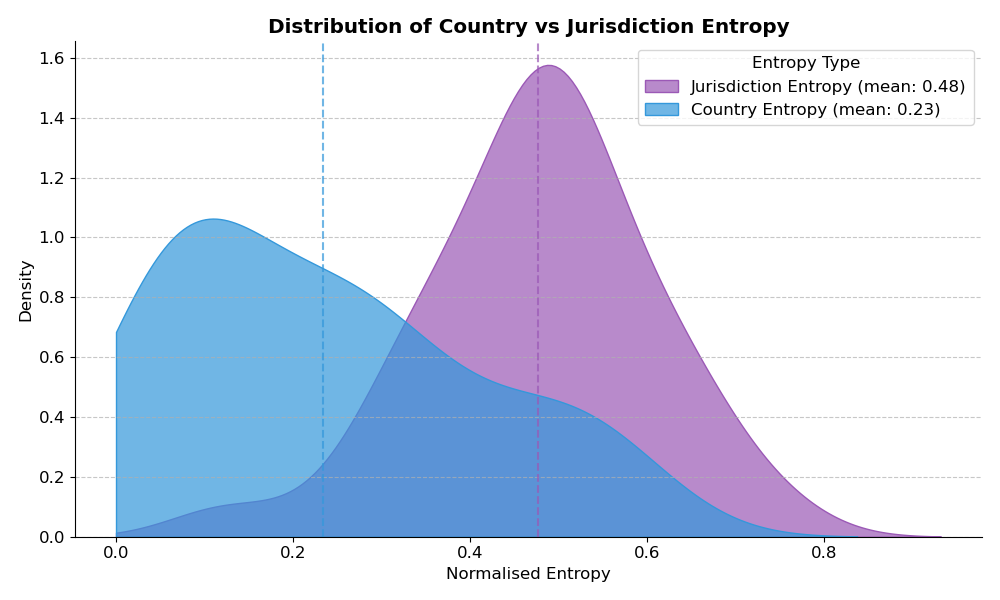
\includegraphics[width=0.8\textwidth]{images/Geography_Country_Level_Entropy_Distribution.png}
    \caption{Distribution of Normalized Entropy for Entity0Countries vs. Incorporation Jurisdictions, Aggregated at the Country Level of Intermediaries}
    \label{fig:geography_country_level_entropy_distribution}
\end{figure}

\subsubsection{Intermediary Specialisation at the Individual Level}
\label{subsubsec:network_countries_served} 

While intermediaries aggregated at the country level exhibit distinct geographical specializations, particularly in their client bases, this section shifts focus to the individual intermediary level. We examine the concentration of countries linked to the entities an individual intermediary serves, and the range of jurisdictions they employ for incorporations.

Figure \ref{fig:geography_distribution_countries_by_intermediary} (left panel) presents the distribution of the number of distinct countries linked to the entities served by each intermediary. The distribution is heavily skewed to the right, with the vast majority of intermediaries (approximately 75\%) serving entities linked to only one country across all the entities it is connected to. More than 90\% of intermediaries are linked to no more than two countries. This indicates that most individual intermediaries, regardless of their home country, focus their client acquisition efforts very narrowly, often within a single national context. The right panel of Figure \ref{fig:geography_distribution_countries_by_intermediary} plots the number of client countries against the log-degree of the intermediary. This scatter plot visually confirms a very low correlation: even intermediaries with a high degree (serving many entities) typically do not serve entities linked to a large number of different countries. This suggests that intermediaries tend to scale their operations by achieving deeper penetration within their existing client geographies rather than by expanding their client base across numerous new countries. This finding aligns with qualitative research suggesting that trust and local network knowledge are paramount in the client-intermediary relationship (Harrington, 2016), favoring localized client acquisition.

\begin{figure}[htbp]
    \centering
    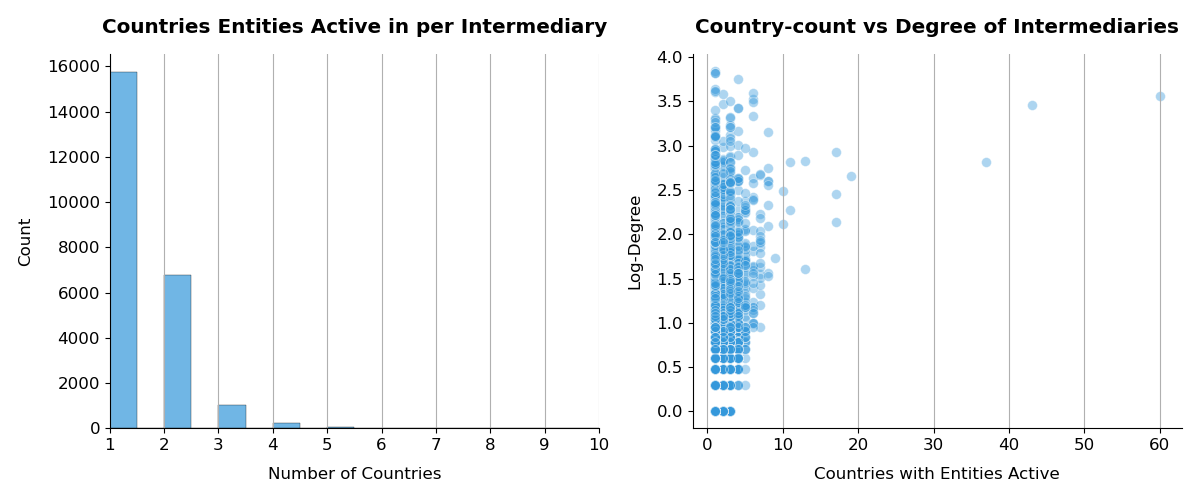
\includegraphics[width=0.9\textwidth]{images/Geography_Distribution_of_Countries_by_Intermediary.png} % Assuming this figure has two panels as described
    \caption{Left: Distribution of the Number of Countries Linked to Entities Served by Intermediary. Right: Scatterplot of Number of Countries vs. Log-Degree of Intermediary}
    \label{fig:geography_distribution_countries_by_intermediary}
\end{figure}

Turning to the jurisdictions used for incorporation, Figure \ref{fig:geography_distribution_jurisdictions_by_intermediary} (left panel) shows the distribution of the number of distinct jurisdictions each intermediary utilizes. Similar to the client country distribution, this is also heavily skewed, with most intermediaries (approximately 65\%) using only one jurisdiction for incorporating entities, and around 85\% using no more than two. This suggests that many intermediaries specialize in the "legal technologies" (Laffitte, 2024) of a very limited number of OFCs. However, comparing this to Figure \ref{fig:geography_distribution_countries_by_intermediary}, the skew appears slightly less extreme, hinting that some intermediaries might use a couple of jurisdictions even if their client base is from a single country. The right panel of Figure \ref{fig:geography_distribution_jurisdictions_by_intermediary} plots the number of jurisdictions used against the log-degree of the intermediary. While still showing considerable concentration, there is a discernible, albeit weak, positive trend: some intermediaries with very high degrees (top 1-5\%) do tend to utilize a broader portfolio of jurisdictions (e.g., 5 or more). This "tail" of highly connected intermediaries who also master a wider range of jurisdictions options may represent a distinct class of "super-enablers" within the offshore system, capable of offering more complex, multi-jurisdictional structuring.

Overall, at the individual level, intermediaries exhibit strong specialization in their client-facing operations, primarily serving entities linked to one or two countries. While many also specialize in using only one or two incorporation jurisdictions, there is a tendency, particularly among larger intermediaries, to command a slightly broader repertoire of jurisdictional tools. This echoes the aggregate finding that the "palette" of incorporation jurisdictions is often wider than the geographical spread of clients, suggesting that even a geographically focused client base may have diverse structuring needs that intermediaries meet by drawing on different OFCs.

\begin{figure}[htbp]
    \centering
    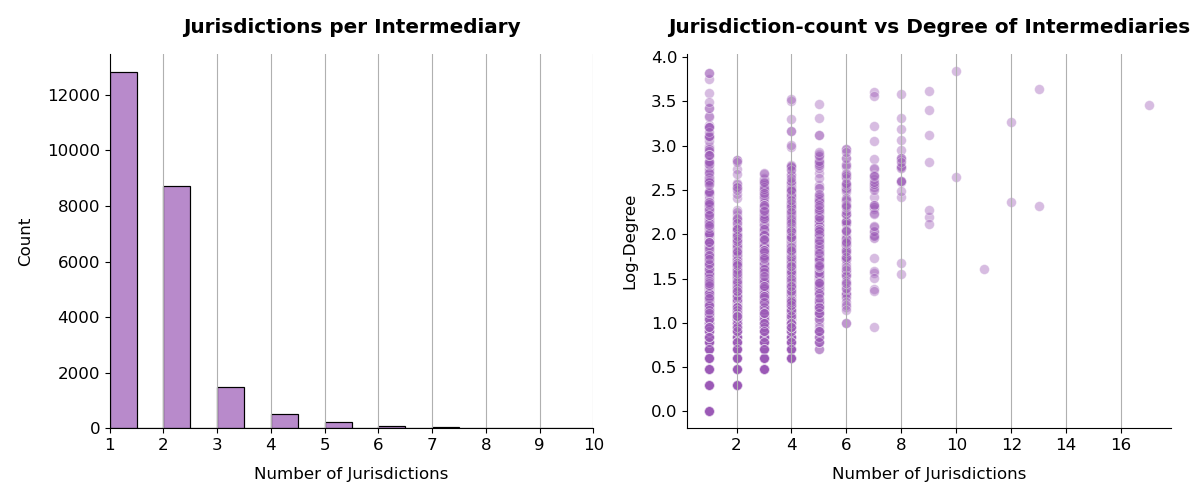
\includegraphics[width=0.9\textwidth]{images/Geography_Distribution_of_Jurisdictions_by_Intermediary.png} % Assuming this figure has two panels
    \caption{Left: Distribution of the Number of Distinct Jurisdictions Used by Intermediary. Right: Scatterplot of Number of Jurisdictions vs. Log-Degree of Intermediary}
    \label{fig:geography_distribution_jurisdictions_by_intermediary}
\end{figure}


\section{Roles and Functions of Intermediaries}
\label{sec:functional_specialisation}

This section transitions from the geographical patterns of intermediary activity to the functional roles within the offshore financial ecosystem. The objective is to understand whether distinct operational characteristics align with the established classifications of intermediary functions from De Groen (2017). 

\subsubsection{Different Levels of Connectivity: Personalised Advice vs. Aid in Incorporation}
\label{subsubsec:connectivity_functional}

A primary hypothesis in differentiating intermediary functions is that their scale of operation, proxied by their network degree, will vary systematically. Intermediaries providing bespoke, personalised advice - such as Tax Experts offering specialised tax planning or Investment Advisors structuring wealth management solutions - will likely serve a smaller number of clients. Conversely, intermediaries whose core function is the more standardized provision of entity incorporation and ongoing administration—such as Administrators and certain Legal Experts specialising in high-volume corporate services - are expected to exhibit higher degrees, indicative of a larger client load.

Figure \ref{fig:specialisation_cdf_degrees} presents the Cumulative Distribution Function (CDF) of degrees for each of the four intermediary classifications within our random sample, plotted on a log-scale - given the power-law distribution of degree noted earlier (see also appendix for reproduction of this core result in this dataset) - to accommodate the wide range. The CDF indicates the proportion of intermediaries (y-axis) whose degree is less than or equal to a given value (x-axis). A curve shifted towards the top-left signifies generally lower degrees.

\begin{figure}[htbp]
    \centering
    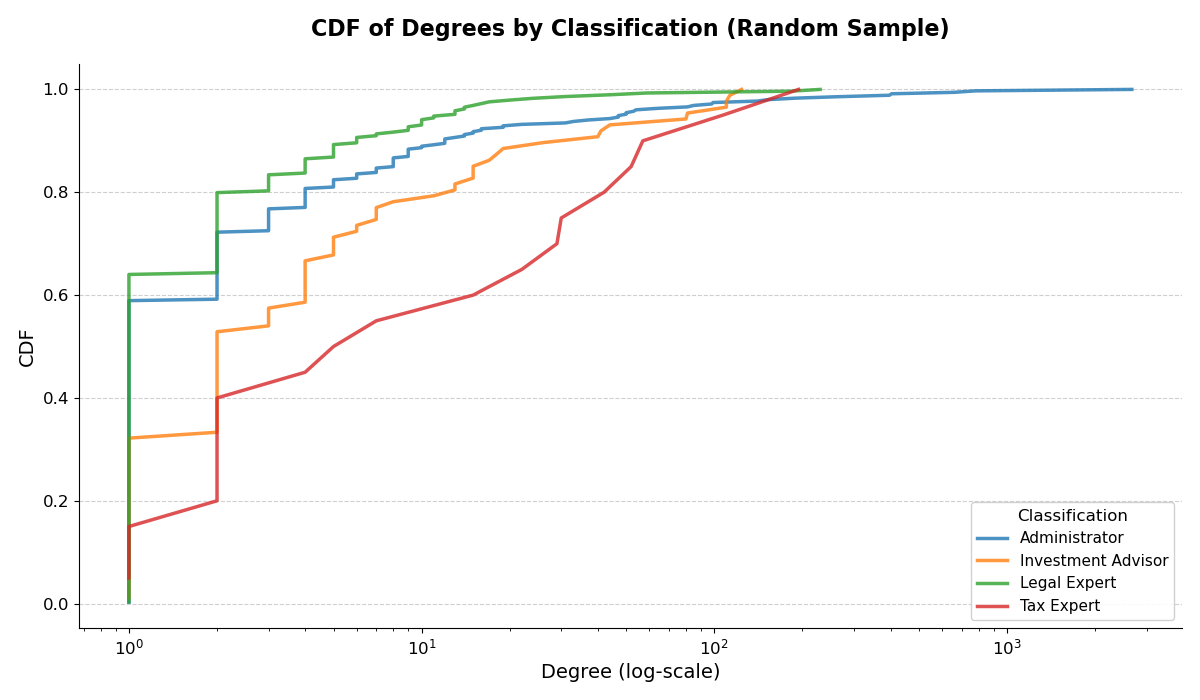
\includegraphics[width=0.8\textwidth]{Specialisation_CDF_of_Degrees_by_Classification_Random_Sample.png}
    \caption{Cumulative Distribution Function (CDF) of Degrees by Intermediary Classification (Random Sample)}
    \label{fig:specialisation_cdf_degrees}
\end{figure}

The plot immediately suggests distinct degree profiles. The CDFs for Tax Experts (green line) and Investment Advisors (orange line) rise very steeply at the lower end of the degree spectrum, indicating that the vast majority of these intermediaries are connected to a relatively small number of entities (e.g., typically fewer than 10). Their curves plateau quickly, showing few instances of high-degree actors in these categories. In contrast, the CDFs for Administrators (blue line) and Legal Experts (red line) rise more gradually and extend further to the right, signifying a broader distribution of degrees, with a considerable proportion of these intermediaries connected to tens, hundreds, or even thousands of entities.

We are again dealing with comparing whether two distributions are significantly different, so we once again turn to the non-parametric two-sample KS test. However, it is a two-sample test, so subsequent pairwise two-sample Kolmogorov-Smirnov (KS) tests were conducted, with a Bonferroni correction applied for the multiple comparisons across the six unique pairs (corrected significance level $\alpha_c = 0.05/6 \approx 0.0083$).  

\begin{itemize}
    \item \textbf{Administrator vs. Investment Advisor:} A significant difference was found ($p \approx 0.0004$), with Administrators exhibiting significantly higher degrees. This supports the hypothesis that administrative services are typically higher volume than bespoke investment advice.
    \item \textbf{Administrator vs. Legal Expert:} No significant difference was detected ($p = 1.0000$). This suggests that, in terms of sheer connectivity, Administrators and Legal Experts in our sample operate at broadly similar scales, likely reflecting the involvement of many Legal Experts in high-volume incorporation and entity management tasks, similar to Administrators.
    \item \textbf{Administrator vs. Tax Expert:} A significant difference was observed ($p \approx 0.0047$, which suggests convincing evidence against the null hypothesis that the observed degrees are sampled from the same underlying distribution. Administrators tend to have higher degrees than Tax Experts, consistent with tax advice being more specialised and lower volume.
    \item \textbf{Investment Advisor vs. Legal Expert:} A significant difference was found ($p < 0.0001$), with Legal Experts having significantly higher degrees. This reinforces the distinction between high-volume legal/incorporation services and lower-volume investment advisory.
    \item \textbf{Investment Advisor vs. Tax Expert:} No significant difference was found ($p = 0.6899$). This lack of difference suggests that Investment Advisors and Tax Experts operate at comparable, generally lower scales of connectivity, consistent with their roles in providing personalised, in-depth advice rather than mass-produced services. 
    \item \textbf{Legal Expert vs. Tax Expert:} A significant difference was detected $p \approx 0.0007$), with Legal Experts typically having higher degrees. This further distinguishes the often high-volume nature of legal services in this context from the more specialised, lower-volume nature of tax expertise.
\end{itemize}

These results broadly support the conceptual division: the "personalised advice" types (Tax Experts and Investment Advisors) tend to have lower degrees and do not significantly differ from each other in connectivity. The "aid in incorporation/management" types (Legal Experts and Administrators) tend to have higher degrees. Comparisons across these two broader functional groups generally reveal significant differences in their scale of operation. But we cannot distinguish between Legal Experts and Administrators in terms of degree, nor Tax Experts and Investment Advisors.

The importance of analysing a random sample, rather than focusing solely on the most connected intermediaries, is underscored by Figure \ref{fig:specialisation_classification_distribution}. This figure compares the distribution of intermediary classifications within our random sample (n=434 after filtering) against a sample composed of the top $\approx$1.5\% of intermediaries by degree (n=345 after filtering). The contrast is stark: the top-degree sample is overwhelmingly dominated by Administrators, who constitute 55.7\% of this group compared to 45.4\% in the random sample. Conversely, Legal Experts (22.6\% in top-degree vs. 29.0\% in random), Investment Advisors (19.1\% vs. 20.5\%), and particularly Tax Experts (a mere 2.6\% vs. 5.1\%) are notably underrepresented among the most connected players. This disparity highlights that an analysis focused only on "super-hub" intermediaries (Kejriwal \& Dang, 2020) would provide a limited and skewed perspective on the functional diversity within the offshore intermediary ecosystem, largely missing the contributions and characteristics of those providing more specialised, lower-volume advisory services. 

\begin{figure}[htbp]
    \centering
    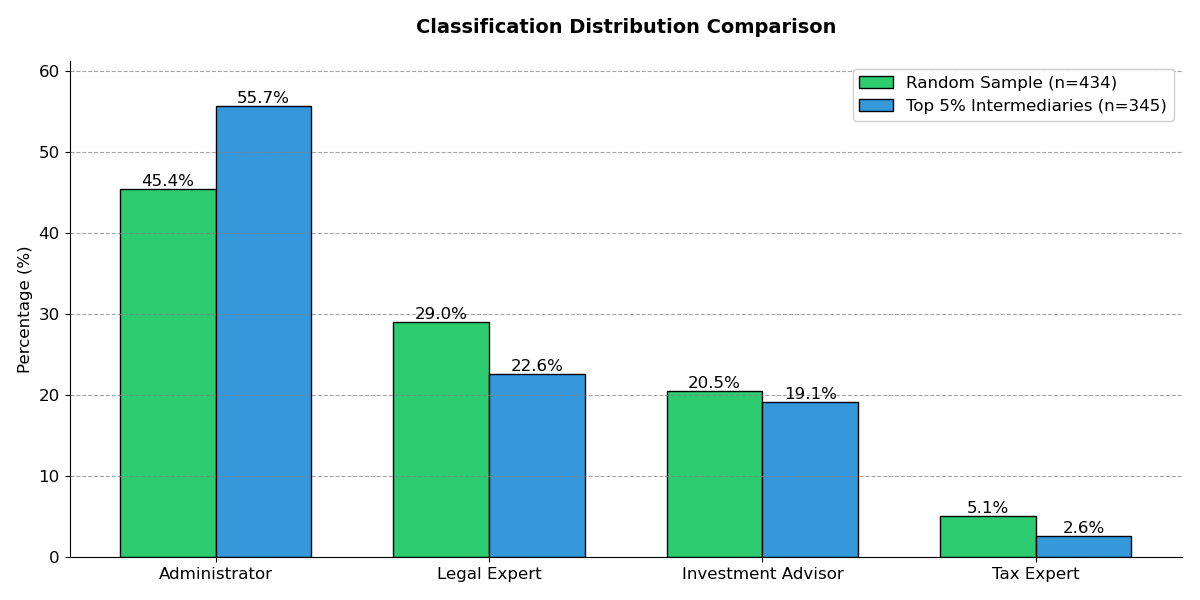
\includegraphics[width=0.8\textwidth]{Specialisation_Classification_Distribution_Comparison.png}
    \caption{Distribution of Intermediary Classifications: Random Sample vs. Top $\approx$1.5\% by Degree}
    \label{fig:specialisation_classification_distribution}
\end{figure}

\subsubsection{Different Activities: Instruments and Service Offerings}
\label{subsubsec:activities_functional}

Beyond sheer connectivity, functional specialisation may also manifest in the nature and diversity of the activities intermediaries undertake. To explore this, we examine five key metrics for each intermediary classification within the random sample:
\begin{enumerate}
    \item \textbf{Jurisdiction Entropy ($H_j$)}: The diversity in the portfolio of jurisdictions where an intermediary incorporates entities. Higher entropy indicates the use of a wider range of jurisdictions.
    \item \textbf{Client Country Entropy ($H_c$)}: The diversity in the countries to which their clients' entities are linked (by activity). Higher entropy suggests a more geographically diverse client base.
    \item \textbf{Regime Entropy}: The diversity in the political regimes (e.g., democracy, autocracy, based on V-Dem data) of the countries where client entities are linked. Higher entropy implies engagement with clients from a broader spectrum of political systems.
    \item \textbf{Legal Technology Entropy}: The diversity in the types of "legal technologies" (as conceptualised by Laffitte, 2024, e.g., specific trust laws, corporate vehicles, secrecy provisions) prevalent in the jurisdictions they use for incorporation. Higher entropy suggests the intermediary leverages a wider array of legal tools available in the global "market for tax havens."
    \item \textbf{Bearer Instrument Usage}: A binary indicator (0 or 1) of whether the intermediary has serviced entities known to have used bearer instruments (e.g., bearer shares), which are high-anonymity tools often associated with obscuring beneficial ownership.
\end{enumerate}

Figure \ref{fig:specialisation_average_entropy_bearer} displays the average values of these metrics for each intermediary classification. Visually, Legal Experts and Administrators tend to show higher average values for most entropy measures, particularly Legal Technology Diversity and Jurisdiction Diversity, compared to Investment Advisors and Tax Experts. Bearer Share Usage appears relatively low across all types, with Tax Experts showing the highest average.

\begin{figure}[htbp]
    \centering
    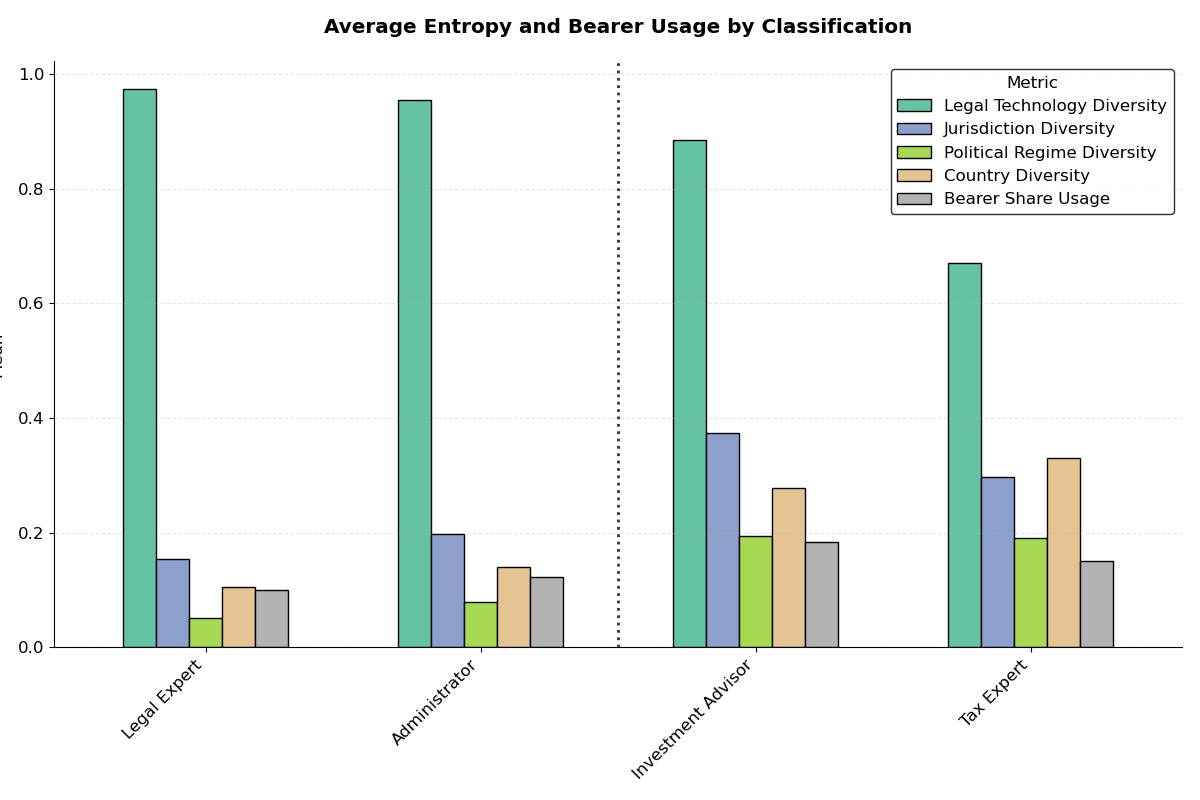
\includegraphics[width=0.9\textwidth]{Specialisation_Average_Entropy_and_Bearer_Usage_by_Classification.png}
    \caption{Average Entropy Measures and Bearer Instrument Usage by Intermediary Classification (Random Sample)}
    \label{fig:specialisation_average_entropy_bearer}
\end{figure}

To formally assess these differences, pairwise comparisons were conducted using Mann-Whitney U tests for the (continuous) entropy measures and Fisher's exact test for the (binary) bearer instrument usage. A Bonferroni correction was applied to account for the 30 comparisons (5 metrics $\times$ 6 unique pairs of classifications), setting the corrected significance threshold at $\alpha_c = 0.05/30 \approx 0.00167$. Key significant findings are summarized below, going measure by measure:

\textbf{Legal Technology Entropy:}
Legal Experts (mean $H_{LT} \approx 0.98$) and Administrators (mean $H_{LT} \approx 0.95$) exhibit significantly higher diversity in the legal technologies of the jurisdictions they utilize compared to Investment Advisors (mean $H_{LT} \approx 0.89$; $p < 0.0001$ vs Legal Experts, $p \approx 0.0047$ vs Administrators) and Tax Experts (mean $H_{LT} \approx 0.67$; $p < 0.0001$ vs Legal Experts, $p < 0.0001$ vs Administrators). This suggests that Legal Experts and Administrators, often involved in the mechanics of entity creation and management across various contexts, engage with a broader array of jurisdictional legal frameworks and offshore "products," as described by Laffitte (2024). No significant difference was found between Legal Experts and Administrators, nor between Investment Advisors and Tax Experts in this regard, reinforcing the two broad functional groupings proposed earlier.

\textbf{Jurisdiction Entropy:}
Legal Experts (mean $H_j \approx 0.15$) show significantly higher diversity in the jurisdictions they use for incorporation compared to Investment Advisors (mean $H_j \approx 0.04$; $p < 0.0001$). Similarly, Administrators (mean $H_j \approx 0.20$) demonstrate greater jurisdiction diversity than Investment Advisors ($p \approx 0.0012$). This indicates that Legal Experts and Administrators tend to draw from a wider palette of offshore jurisdictions when structuring entities for their clients, which aligns with their higher connectivity and broader operational scope. Other pairwise comparisons for jurisdiction entropy did not yield statistically significant differences after Bonferroni correction.

\textbf{Regime Entropy:}
Legal Experts (mean $H_{Regime} \approx 0.05$) exhibit significantly higher diversity in the political regimes of their client countries compared to Investment Advisors (mean $H_{Regime} \approx 0.02$; $p < 0.0001$) and Tax Experts (mean $H_{Regime} \approx 0.02$; $p \approx 0.0001$). Administrators (mean $H_{Regime} \approx 0.08$) also show significantly higher regime diversity than Investment Advisors ($p \approx 0.0044$). This pattern suggests that Legal Experts and Administrators may cater to clienteles originating from, or structuring activities in, a more diverse set of political environments, potentially reflecting more internationalized operations.

\textbf{Client Country Entropy:}
Legal Experts (mean $H_c \approx 0.10$) demonstrate significantly higher diversity in their client countries compared to Investment Advisors (mean $H_c \approx 0.03$; $p \approx 0.0001$) and Tax Experts (mean $H_c \approx 0.03$; $p < 0.0001$). Administrators (mean $H_c \approx 0.14$) also have significantly more diverse client countries than Tax Experts ($p \approx 0.0057$). This implies that Legal Experts, and to some extent Administrators, engage with clients whose activities span a broader range of countries, consistent with their roles in facilitating complex, multi-jurisdictional structures for a larger number of entities.

\textbf{Bearer Instrument Usage:}
After Bonferroni correction, \textbf{no statistically significant differences} were found in the propensity to use bearer instruments among any of the intermediary classifications (e.g., Administrator vs. Tax Expert, Fisher's exact $p \approx 0.13$). While Tax Experts show a slightly higher raw average usage in Figure \ref{fig:specialisation_average_entropy_bearer}, this difference is not statistically significant. This suggests that, within this classified random sample, the use of these high-anonymity instruments is not strongly associated with a particular functional type of intermediary. Their seemingly non-specialised use might imply either a more diffuse deployment across the offshore industry for specific client needs.

The activity metrics, therefore, largely reinforce the distinctions observed in connectivity. Legal Experts and Administrators, typically more connected, also tend to exhibit greater diversity across various geographical, political regime, and legal-technical dimensions of their service offerings - all measures, it should be noted, that are likely to be closely correlated between themselves. This is consistent with their roles in high-volume incorporation and management, potentially serving more international and varied clienteles or requiring a broader toolkit of jurisdictional solutions. The "personalised advice" groups (Tax Experts and Investment Advisors), with their lower connectivity, generally appear more focused in these activity respects. 

